% ====================================================================
% JAISP talk -- Roman Science Conference, Caltech/IPAC, July 13-16 2026
% 15-minute talk (~12 min + questions).
% Build:  latexmk -pdf jaisp_roman_talk.tex
% Figures are pulled directly from ../../paper/figures/
% ====================================================================
\documentclass[aspectratio=169,10pt]{beamer}

\usepackage{graphicx}
\usepackage{booktabs}
\usepackage{amsmath,amssymb}
\graphicspath{{../../paper/figures/}}

% --- clean look ---
\usetheme{default}
\usecolortheme{seagull}
\setbeamertemplate{navigation symbols}{}
\setbeamertemplate{itemize items}[circle]
\setbeamertemplate{itemize subitem}[circle]

\definecolor{jaispblue}{RGB}{20,60,110}
\definecolor{jaispteal}{RGB}{0,120,130}
\definecolor{jaispaccent}{RGB}{190,70,25}
\setbeamercolor{frametitle}{fg=white,bg=jaispblue}
\setbeamercolor{title}{fg=jaispblue}
\setbeamercolor{structure}{fg=jaispblue}
\setbeamercolor{alerted text}{fg=jaispaccent}
\setbeamerfont{frametitle}{series=\bfseries,size=\large}
\setbeamertemplate{frametitle}{%
  \vspace*{0.25em}%
  \begin{beamercolorbox}[wd=\paperwidth,sep=0.5em]{frametitle}%
    \insertframetitle\hfill{\normalfont\small\insertframenumber/\inserttotalframenumber}%
  \end{beamercolorbox}}

\newcommand{\jaisp}{\textsc{Jaisp}}
\newcommand{\mas}{\,\mathrm{mas}}
\newcommand{\srcnote}[1]{{\tiny\textcolor{gray}{#1}}}

\title{{\Huge\jaisp}\\[0.5em]
  \Large A Joint Rubin--\textit{Euclid} Foundation Model for Detection and Astrometry\\[0.3em]
  \large --- and a path to \textit{Roman} ---}
\author{Shoubaneh Hemmati\\[0.3em]
  {\small with G.\ Helou, Y.-H.\ Lin, R.\ Akeson, C.\,D.\ Dowell, A.\ Faisst, T.\ Greene, D.\ Shupe}}
\institute{IPAC, California Institute of Technology}
\date{Roman Science Conference $\cdot$ Caltech/IPAC $\cdot$ July 2026}

\begin{document}

% ------------------------------------------------------------ 1
\begin{frame}[plain]
  \titlepage
  \vfill
  \centering
  \srcnote{Hemmati et al.\ 2026, submitted to ApJ \quad$\cdot$\quad code: github.com/xoubish/JAISP}
\end{frame}

% ------------------------------------------------------------ 2
\begin{frame}{Why combine surveys at the pixel level?}
  \begin{itemize}\setlength\itemsep{0.7em}
    \item Cosmology is now limited by \alert{systematics, not statistics}: residual tensions
      between probes can neither be dismissed as noise nor attributed to new physics.
    \item Rubin/LSST, \textit{Euclid}, and \textit{Roman} will observe overlapping sky from
      ${\sim}0.3$ to $2\,\mu$m at sub-arcsecond resolution --- in combination they can
      \alert{calibrate and cross-check one another}, suppressing survey-specific systematics
      no single survey can control alone.
    \item But joint pixel-level processing means confronting \alert{heterogeneous PSFs,
      samplings, depths, and noise} simultaneously --- a regime where classical
      pipelines strain.
    \item Classical pipelines encode decades of problem-specific effort. The goal is not to
      discard them, but to move the \emph{joint, cross-instrument} part of the problem into a
      representation \alert{learned from the pixels themselves}.
  \end{itemize}
\end{frame}

% ------------------------------------------------------------ 3
\begin{frame}{The foundation-model recipe: one representation, many cheap heads}
  \begin{columns}[T]
    \begin{column}{0.58\textwidth}
      \textbf{Train once, self-supervised:}
      \begin{itemize}
        \item masked-band autoencoder --- hide one of the ten bands, predict it from the other nine
        \item \alert{no labels, no catalogs} --- raw public mosaics only
      \end{itemize}
      \vspace{0.5em}
      \textbf{Freeze, then reuse:}
      \begin{itemize}
        \item every measurement is a small head ($\lesssim$ few M parameters) reading cached frozen features
        \item detection \& astrometry in hand; photometry \& shapes in preparation
      \end{itemize}
    \end{column}
    \begin{column}{0.38\textwidth}
      \begin{beamercolorbox}[sep=0.8em,rounded=true]{block body}
        \textbf{Cost structure}\\[0.4em]
        Pretraining: \alert{${\sim}2.5$ GPU-hours}\\[0.2em]
        Model size: ${\sim}9$M parameters\\[0.2em]
        Features: extracted once per dataset\\[0.2em]
        Each new task: a small head on cached features\\[0.4em]
        {\small $\Rightarrow$ marginal cost per task $\to$ small; per field $\to$ zero (as we will see)}
      \end{beamercolorbox}
    \end{column}
  \end{columns}
\end{frame}

% ------------------------------------------------------------ 4
\begin{frame}{Data: the earliest public release of each survey}
  \centering
  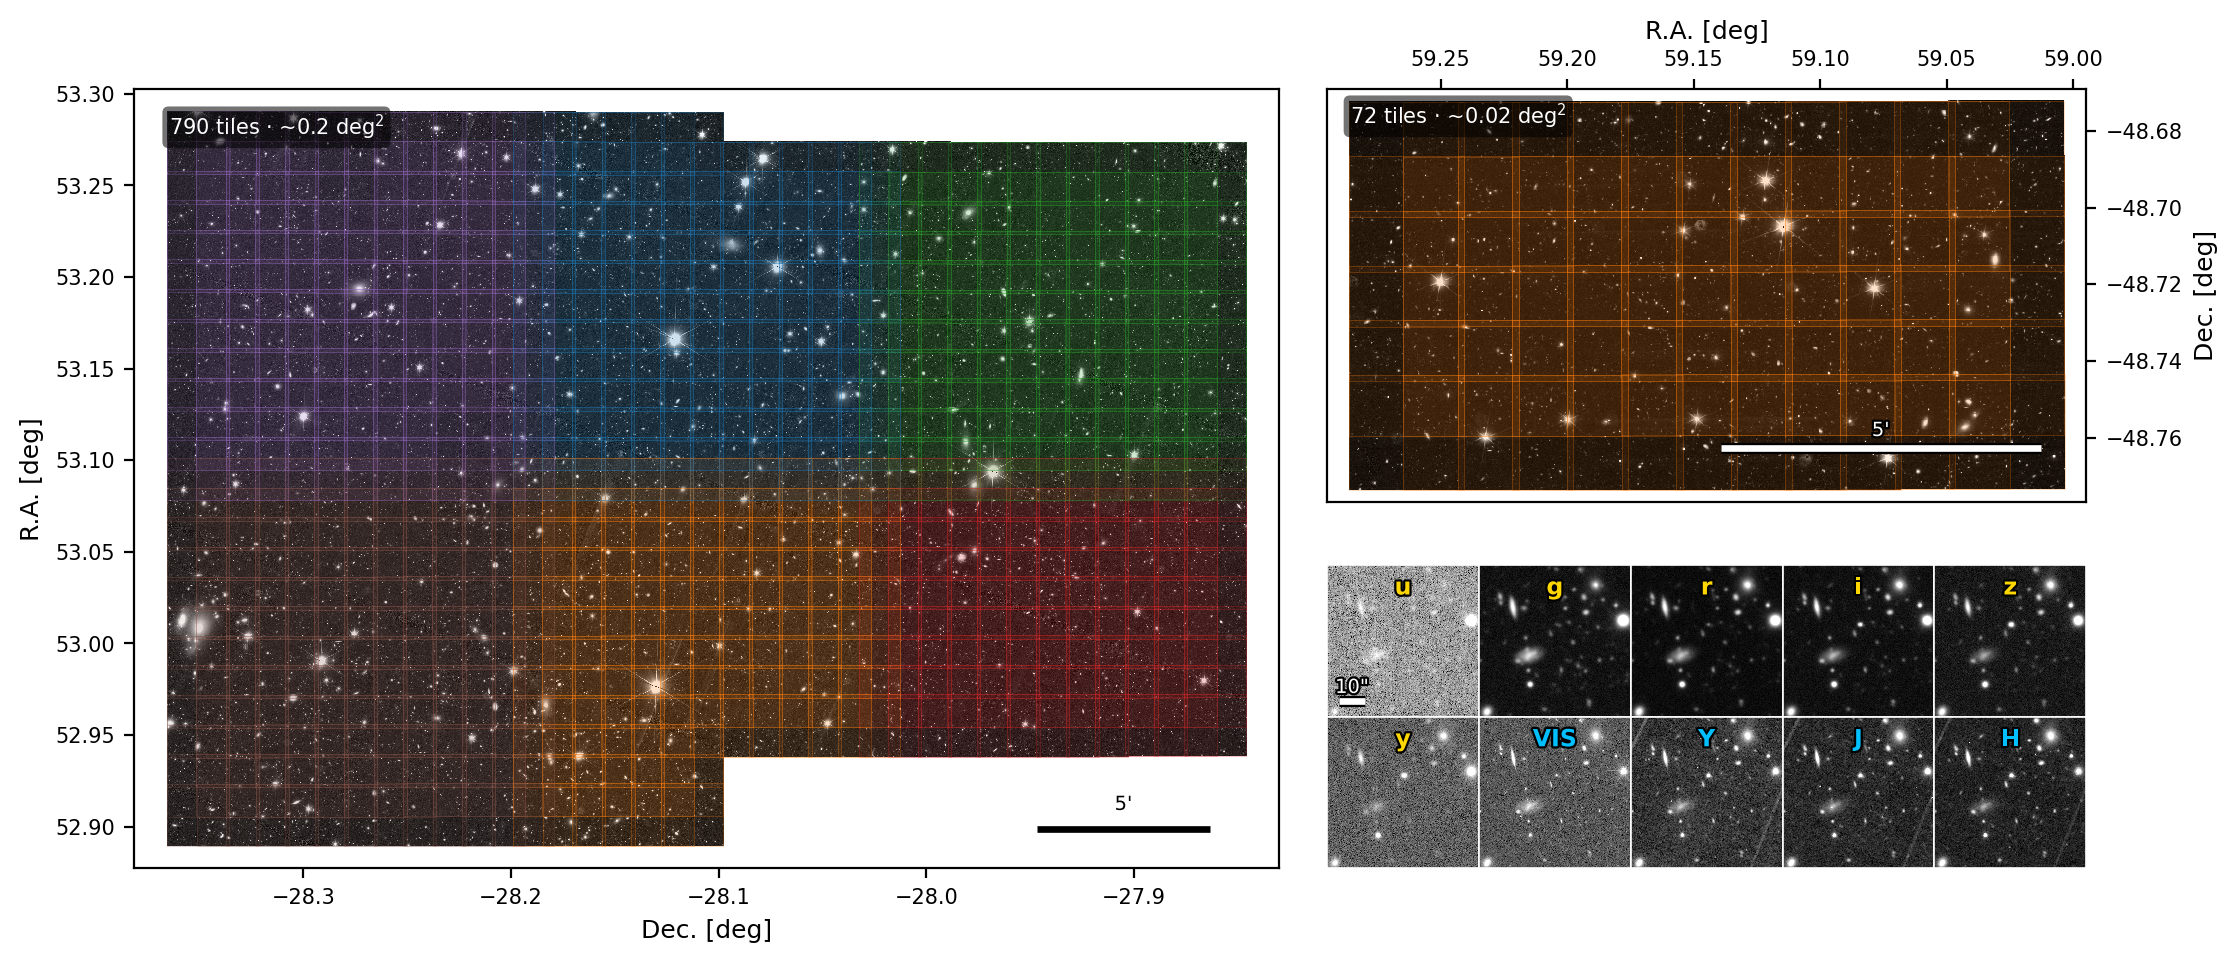
\includegraphics[width=0.86\textwidth]{fig1_data.png}
  \begin{itemize}\small
    \item \textbf{Rubin DP1} (ComCam commissioning, $ugrizy$ at $0.2''$/px, PSF ${\sim}1''$)
      $+$ \textbf{\textit{Euclid} Q1} MER mosaics (VIS $+$ NISP $YJH$ at $0.1''$/px).
    \item Training: 790 matched ten-band tiles over ${\sim}0.2\,\mathrm{deg}^2$ of ECDFS/EDF-Fornax.
      \alert{EDF-S held out entirely} for the transfer test.
  \end{itemize}
\end{frame}

% ------------------------------------------------------------ 5
\begin{frame}{Architecture: each instrument at its native resolution}
  \centering
  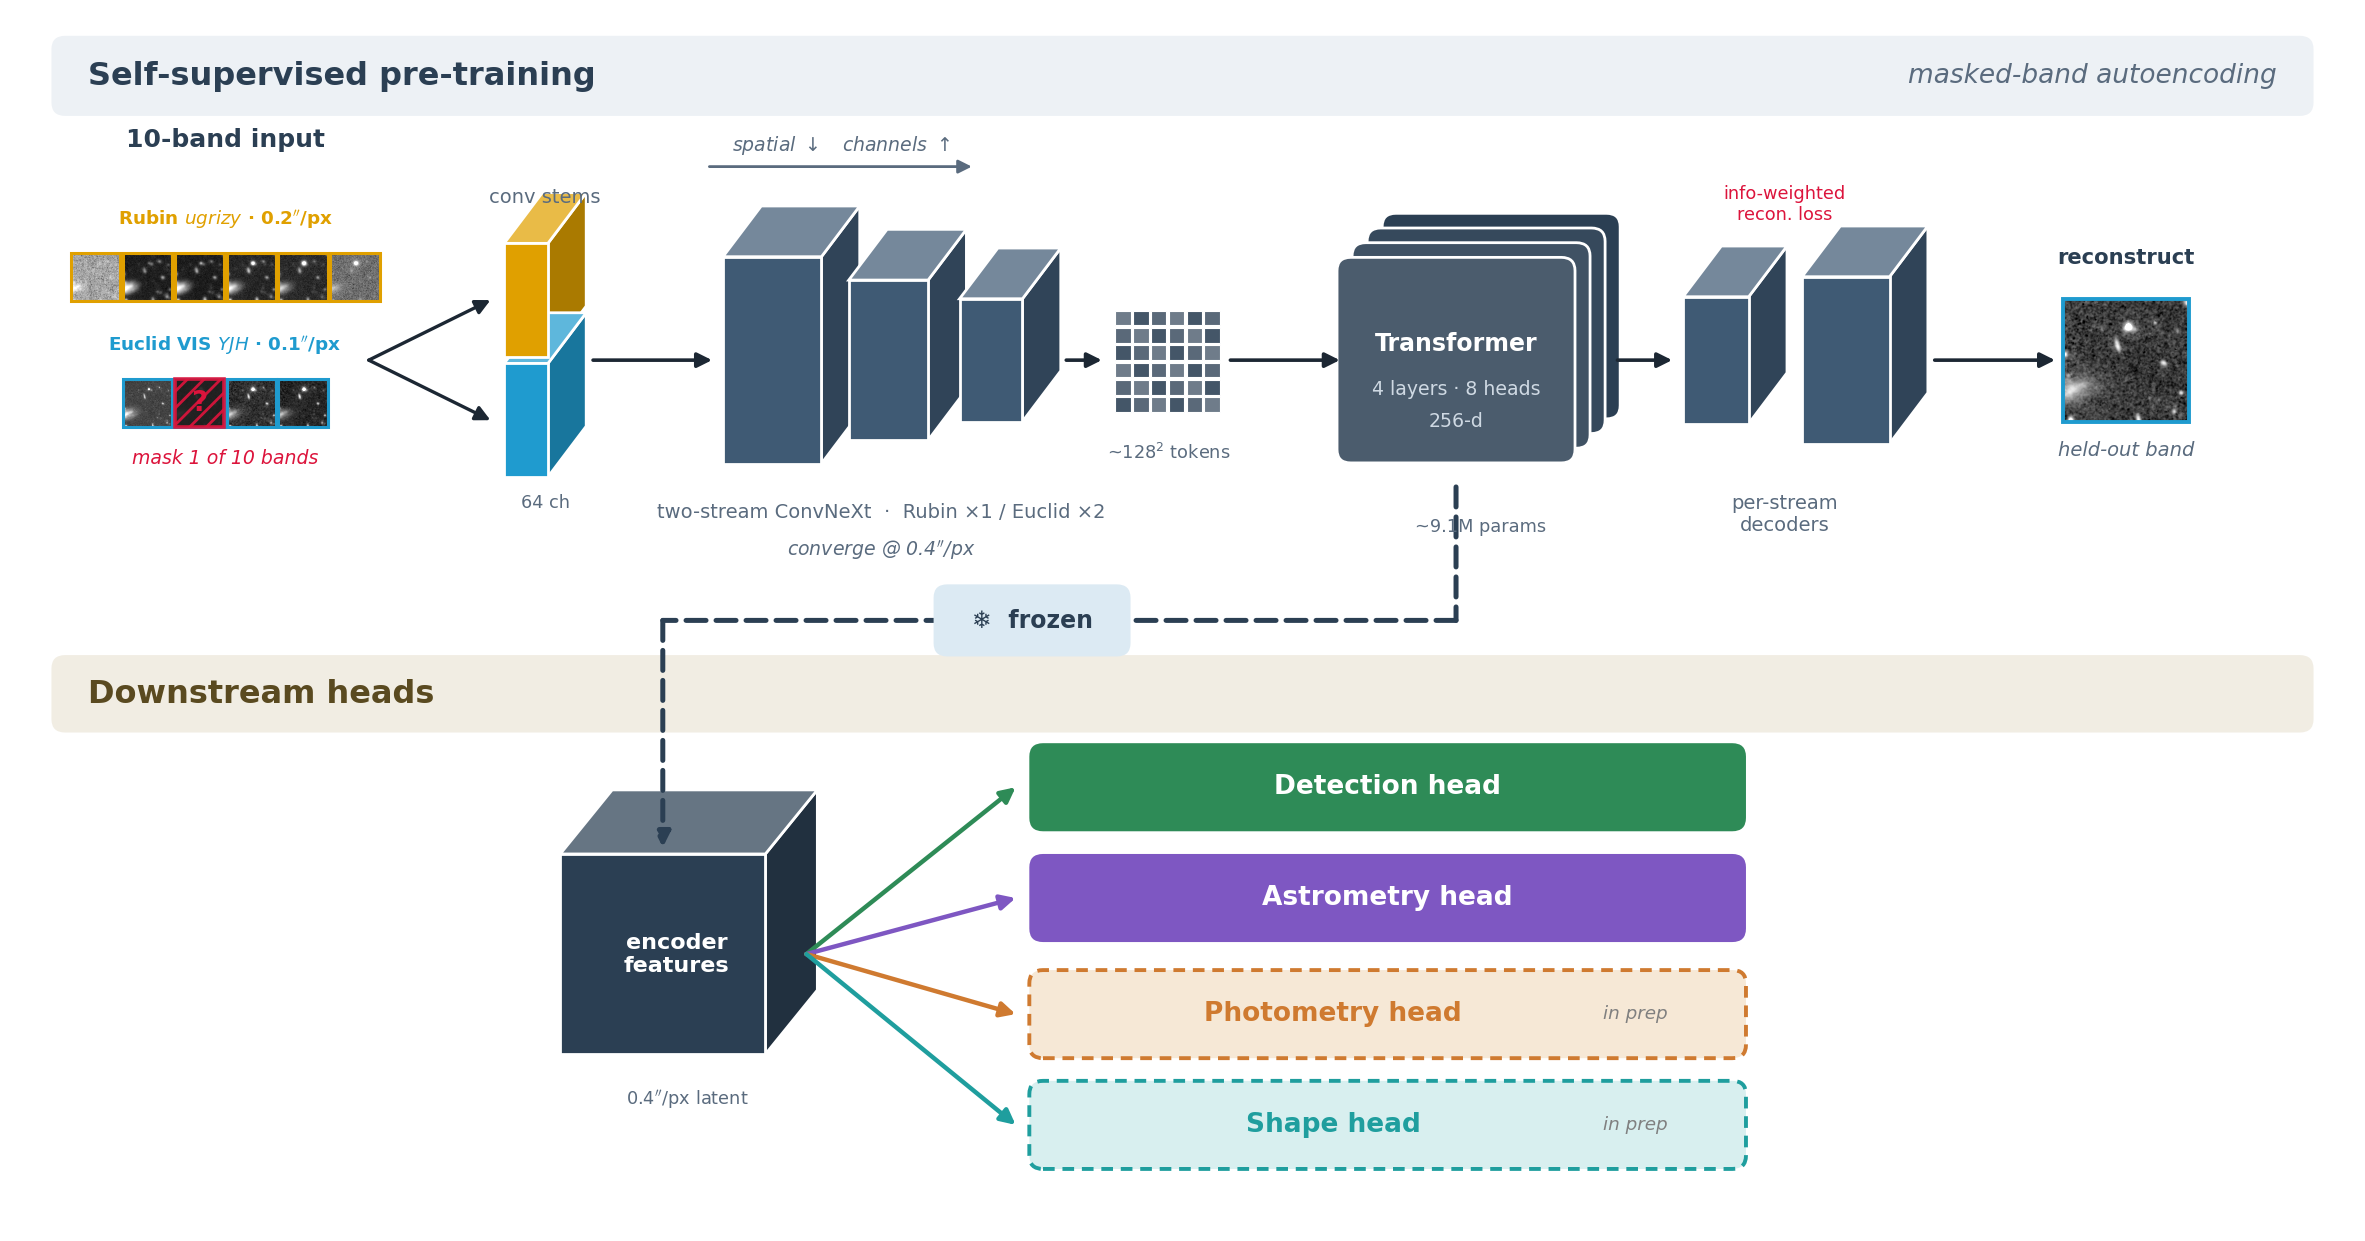
\includegraphics[width=0.80\textwidth]{fig2_architecture.png}
  \begin{itemize}\small
    \item Per-band stems $\to$ two encoder branches (Rubin at $0.2''$, \textit{Euclid} at $0.1''$)
      $\to$ fused on a common $0.4''$ grid $\to$ transformer bottleneck mixes all ten bands.
    \item \alert{Why reconstruction, not alignment?} Contrastive/JEPA objectives reward
      \emph{similar} features but never require \emph{where} --- pixel reconstruction forces
      sub-pixel spatial layout to survive into the representation.
  \end{itemize}
\end{frame}

% ------------------------------------------------------------ 6
\begin{frame}{Did it learn cross-instrument structure?}
  \begin{columns}[T]
    \begin{column}{0.46\textwidth}
      \centering
      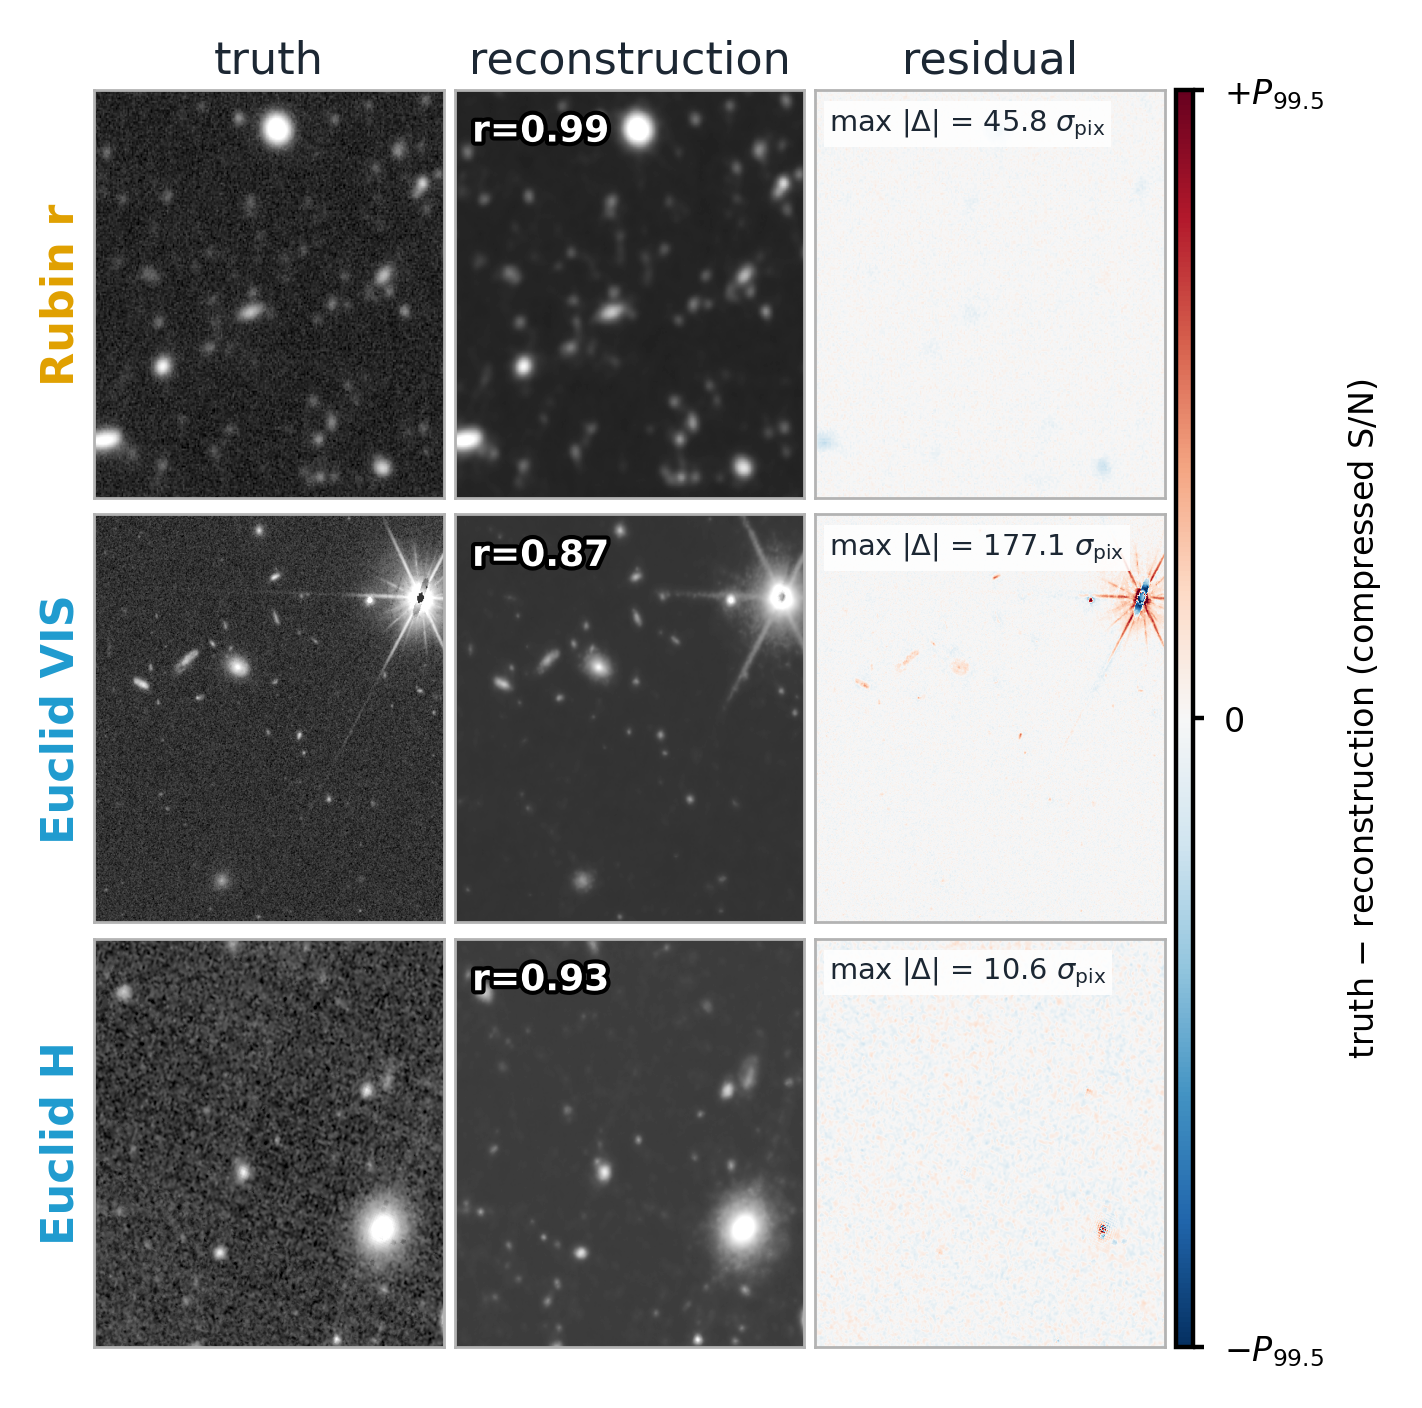
\includegraphics[height=0.72\textheight]{fig3_reconstruction.png}
    \end{column}
    \begin{column}{0.52\textwidth}
      \vspace{1.5em}
      \begin{itemize}\setlength\itemsep{0.8em}
        \item Held-out tiles: withhold one band, predict it from the other nine.
        \item Rubin $r$, \textit{Euclid} VIS, and NISP $H$ all reconstructed faithfully ---
          residuals confined to bright cores and faint galaxy wings.
        \item A band from \alert{one instrument predicted from bands of the other}:
          genuine cross-instrument correspondence, not within-instrument copying.
      \end{itemize}
    \end{column}
  \end{columns}
\end{frame}

% ------------------------------------------------------------ 7
\begin{frame}{...and is it organized physically?}
  \centering
  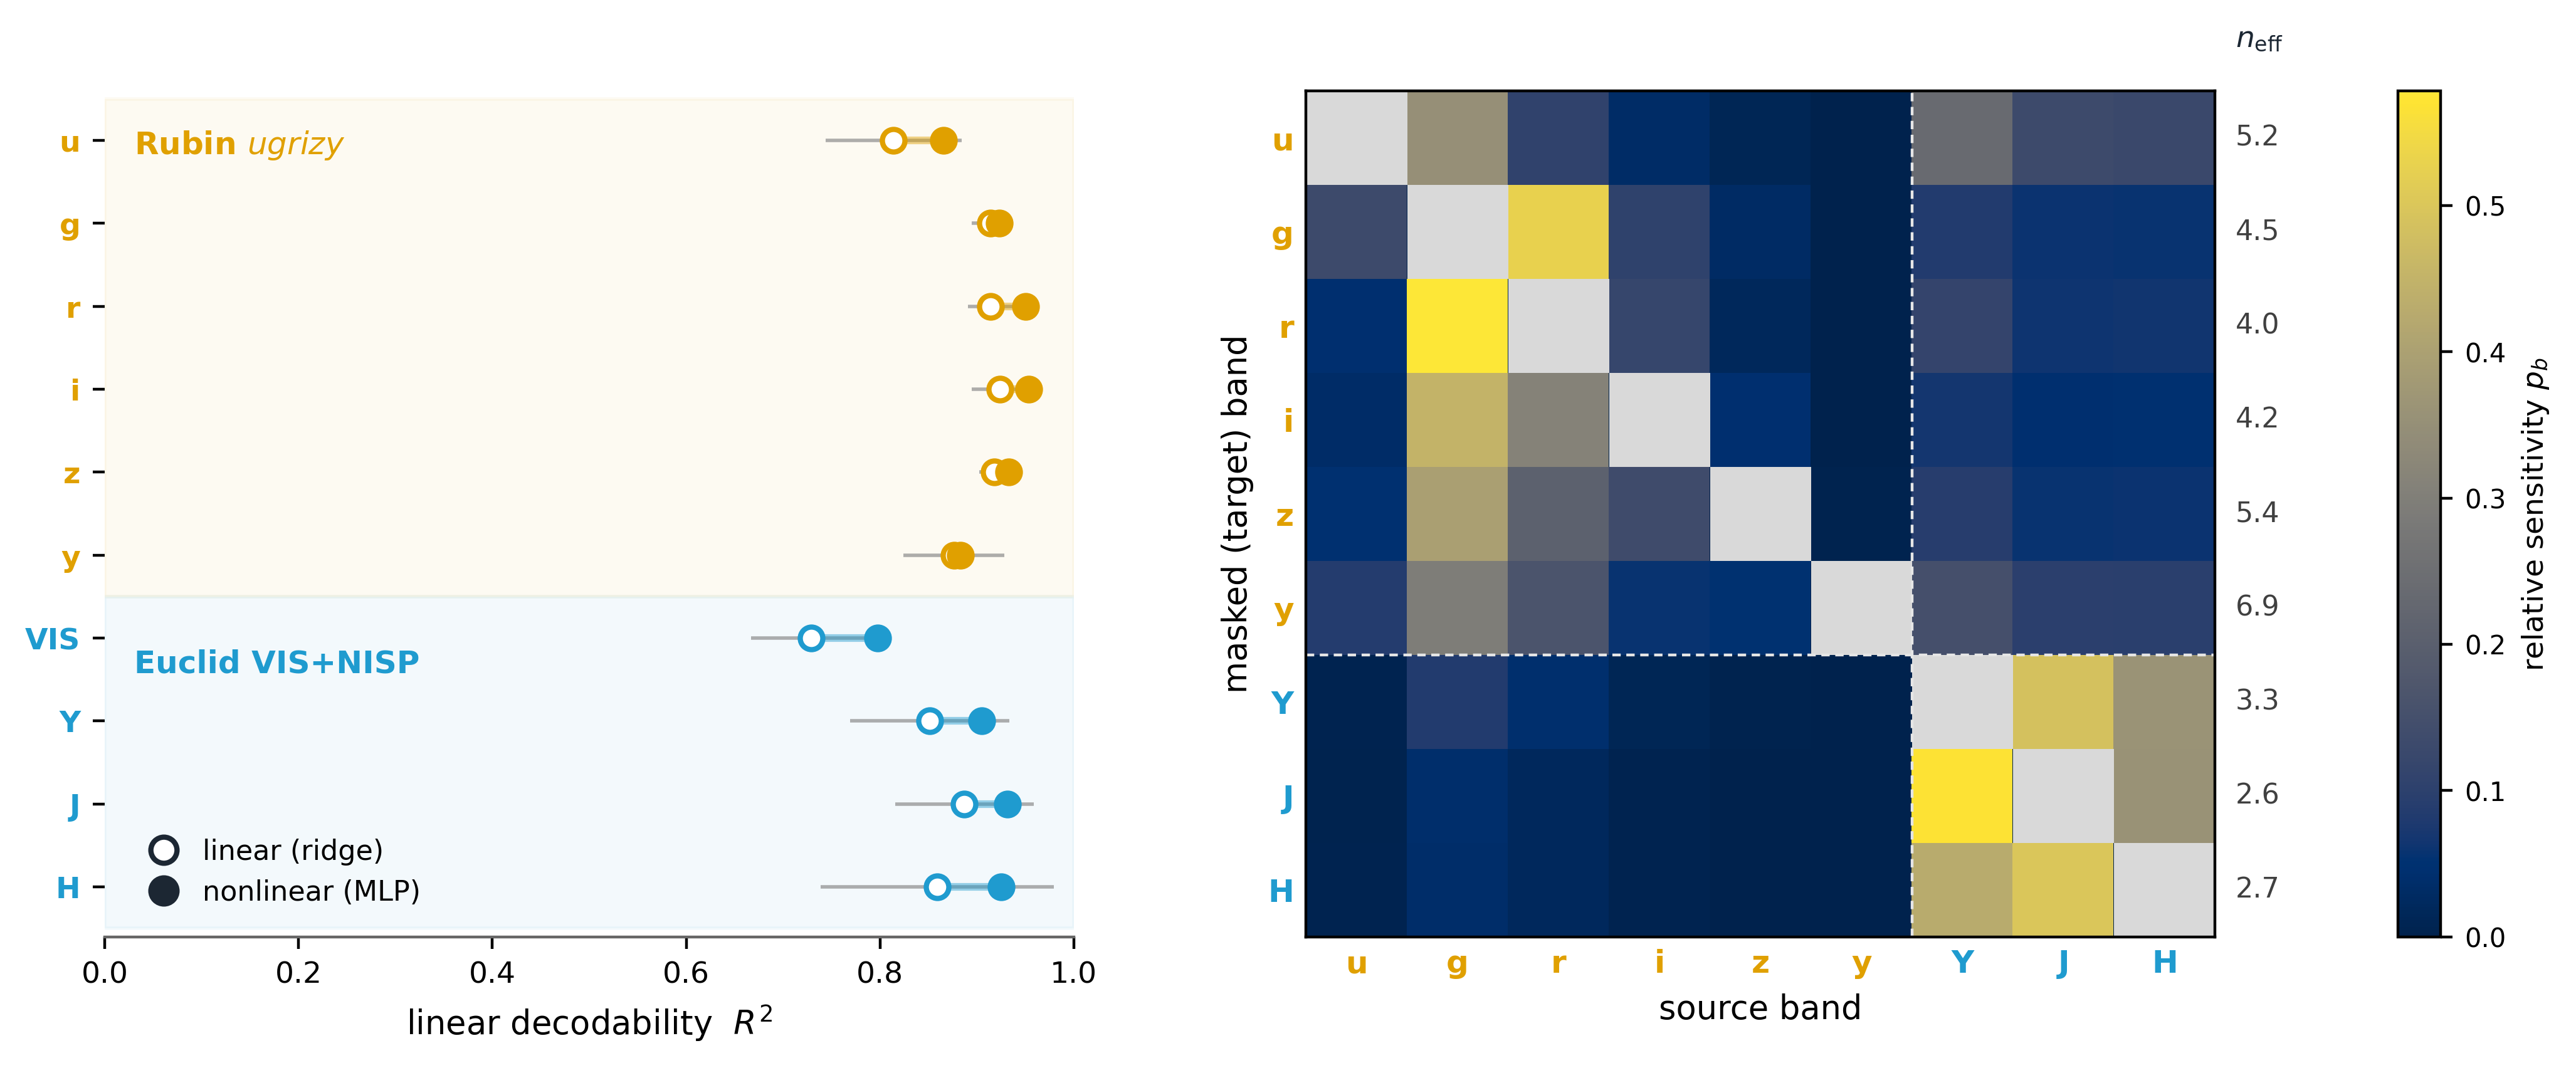
\includegraphics[width=0.88\textwidth]{fig4_probe.png}
  \begin{itemize}\small
    \item \textbf{Left:} every band's brightness is \alert{linearly decodable} from the frozen
      features ($R^2 \approx 0.7$--$0.95$) --- accessible to any downstream head.
    \item \textbf{Right:} information routing mirrors real SEDs: VIS acts as the universal
      spatial scaffold; Rubin bands draw on spectral neighbors; NISP $YJH$ form a
      near-closed block.
  \end{itemize}
\end{frame}

% ------------------------------------------------------------ 8
\begin{frame}{Downstream task 1 --- Detection}
  \centering
  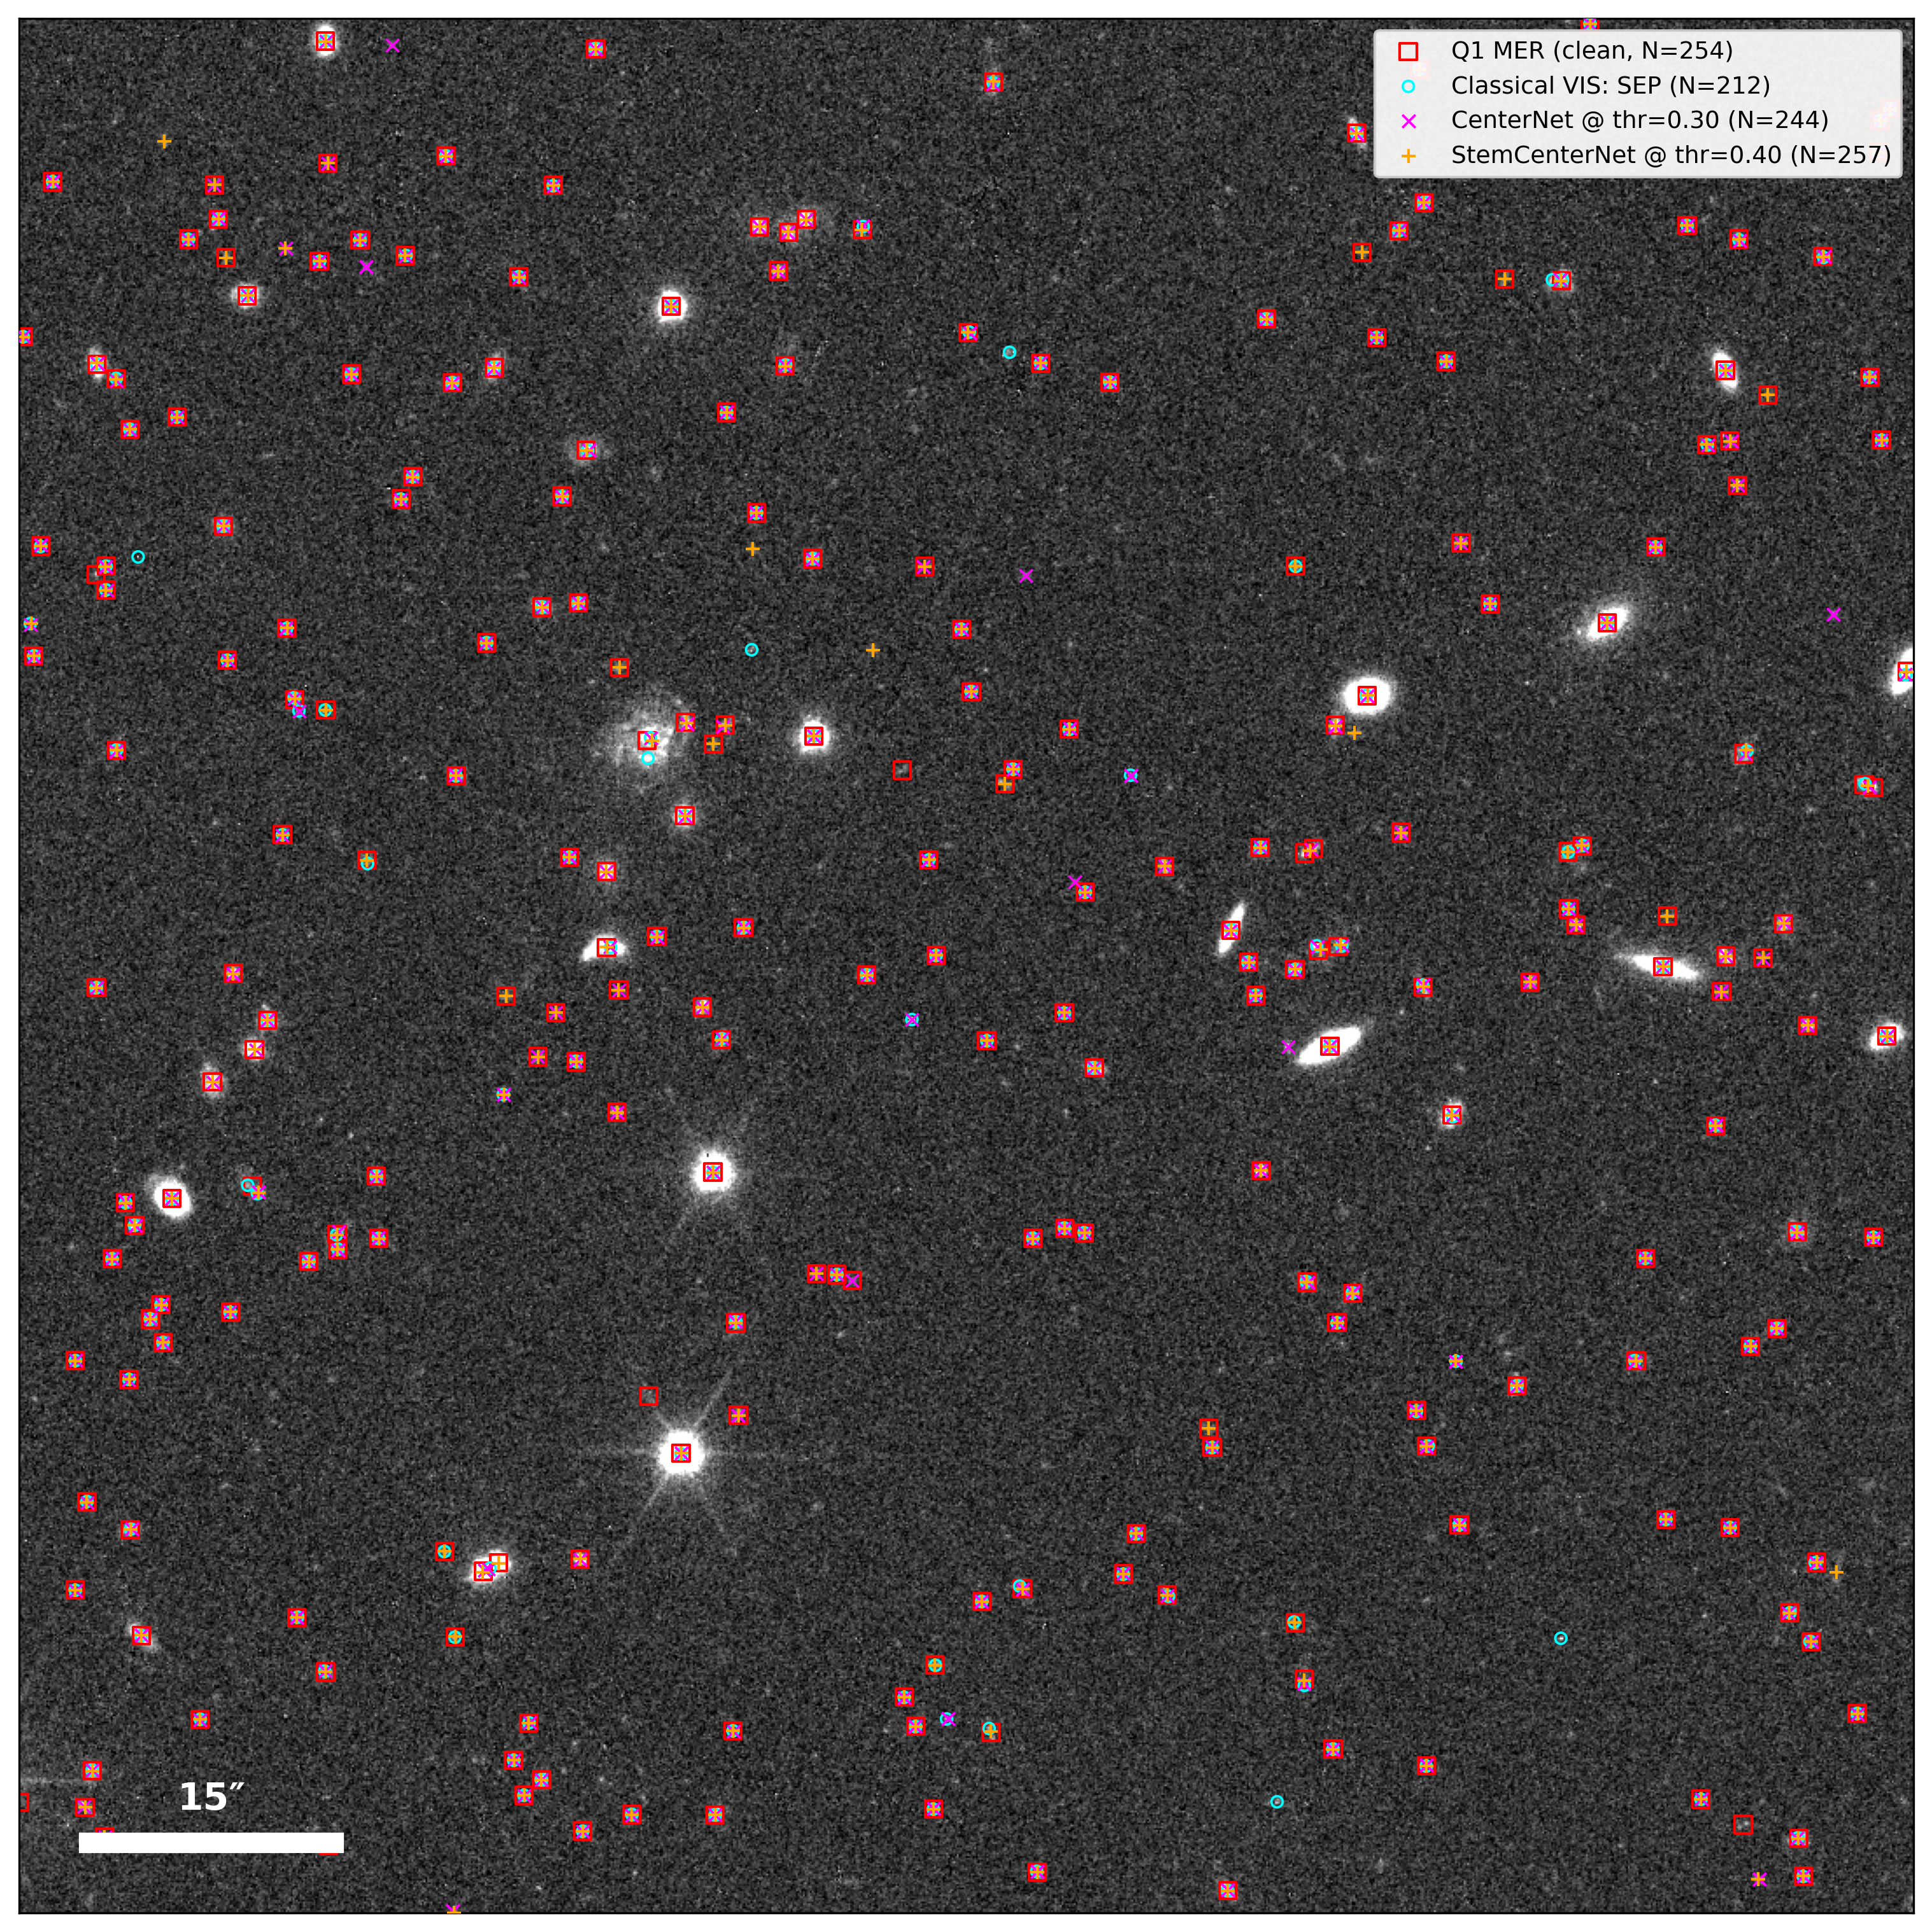
\includegraphics[height=0.60\textheight]{fig5_detection.png}
  \begin{itemize}\small
    \item A CenterNet-style head on the frozen fused features, trained on \alert{lightweight
      classical labels} (SEP $3\sigma$ on VIS) --- no curated catalog supervision.
    \item Matches the \textit{Euclid} Q1 MER catalog on held-out sky; returns
      \alert{one detection per galaxy} where classical extraction fragments extended systems.
  \end{itemize}
\end{frame}

% ------------------------------------------------------------ 9
\begin{frame}{Detection: ten bands buy real depth}
  \begin{columns}[T]
    \begin{column}{0.60\textwidth}
      \centering
      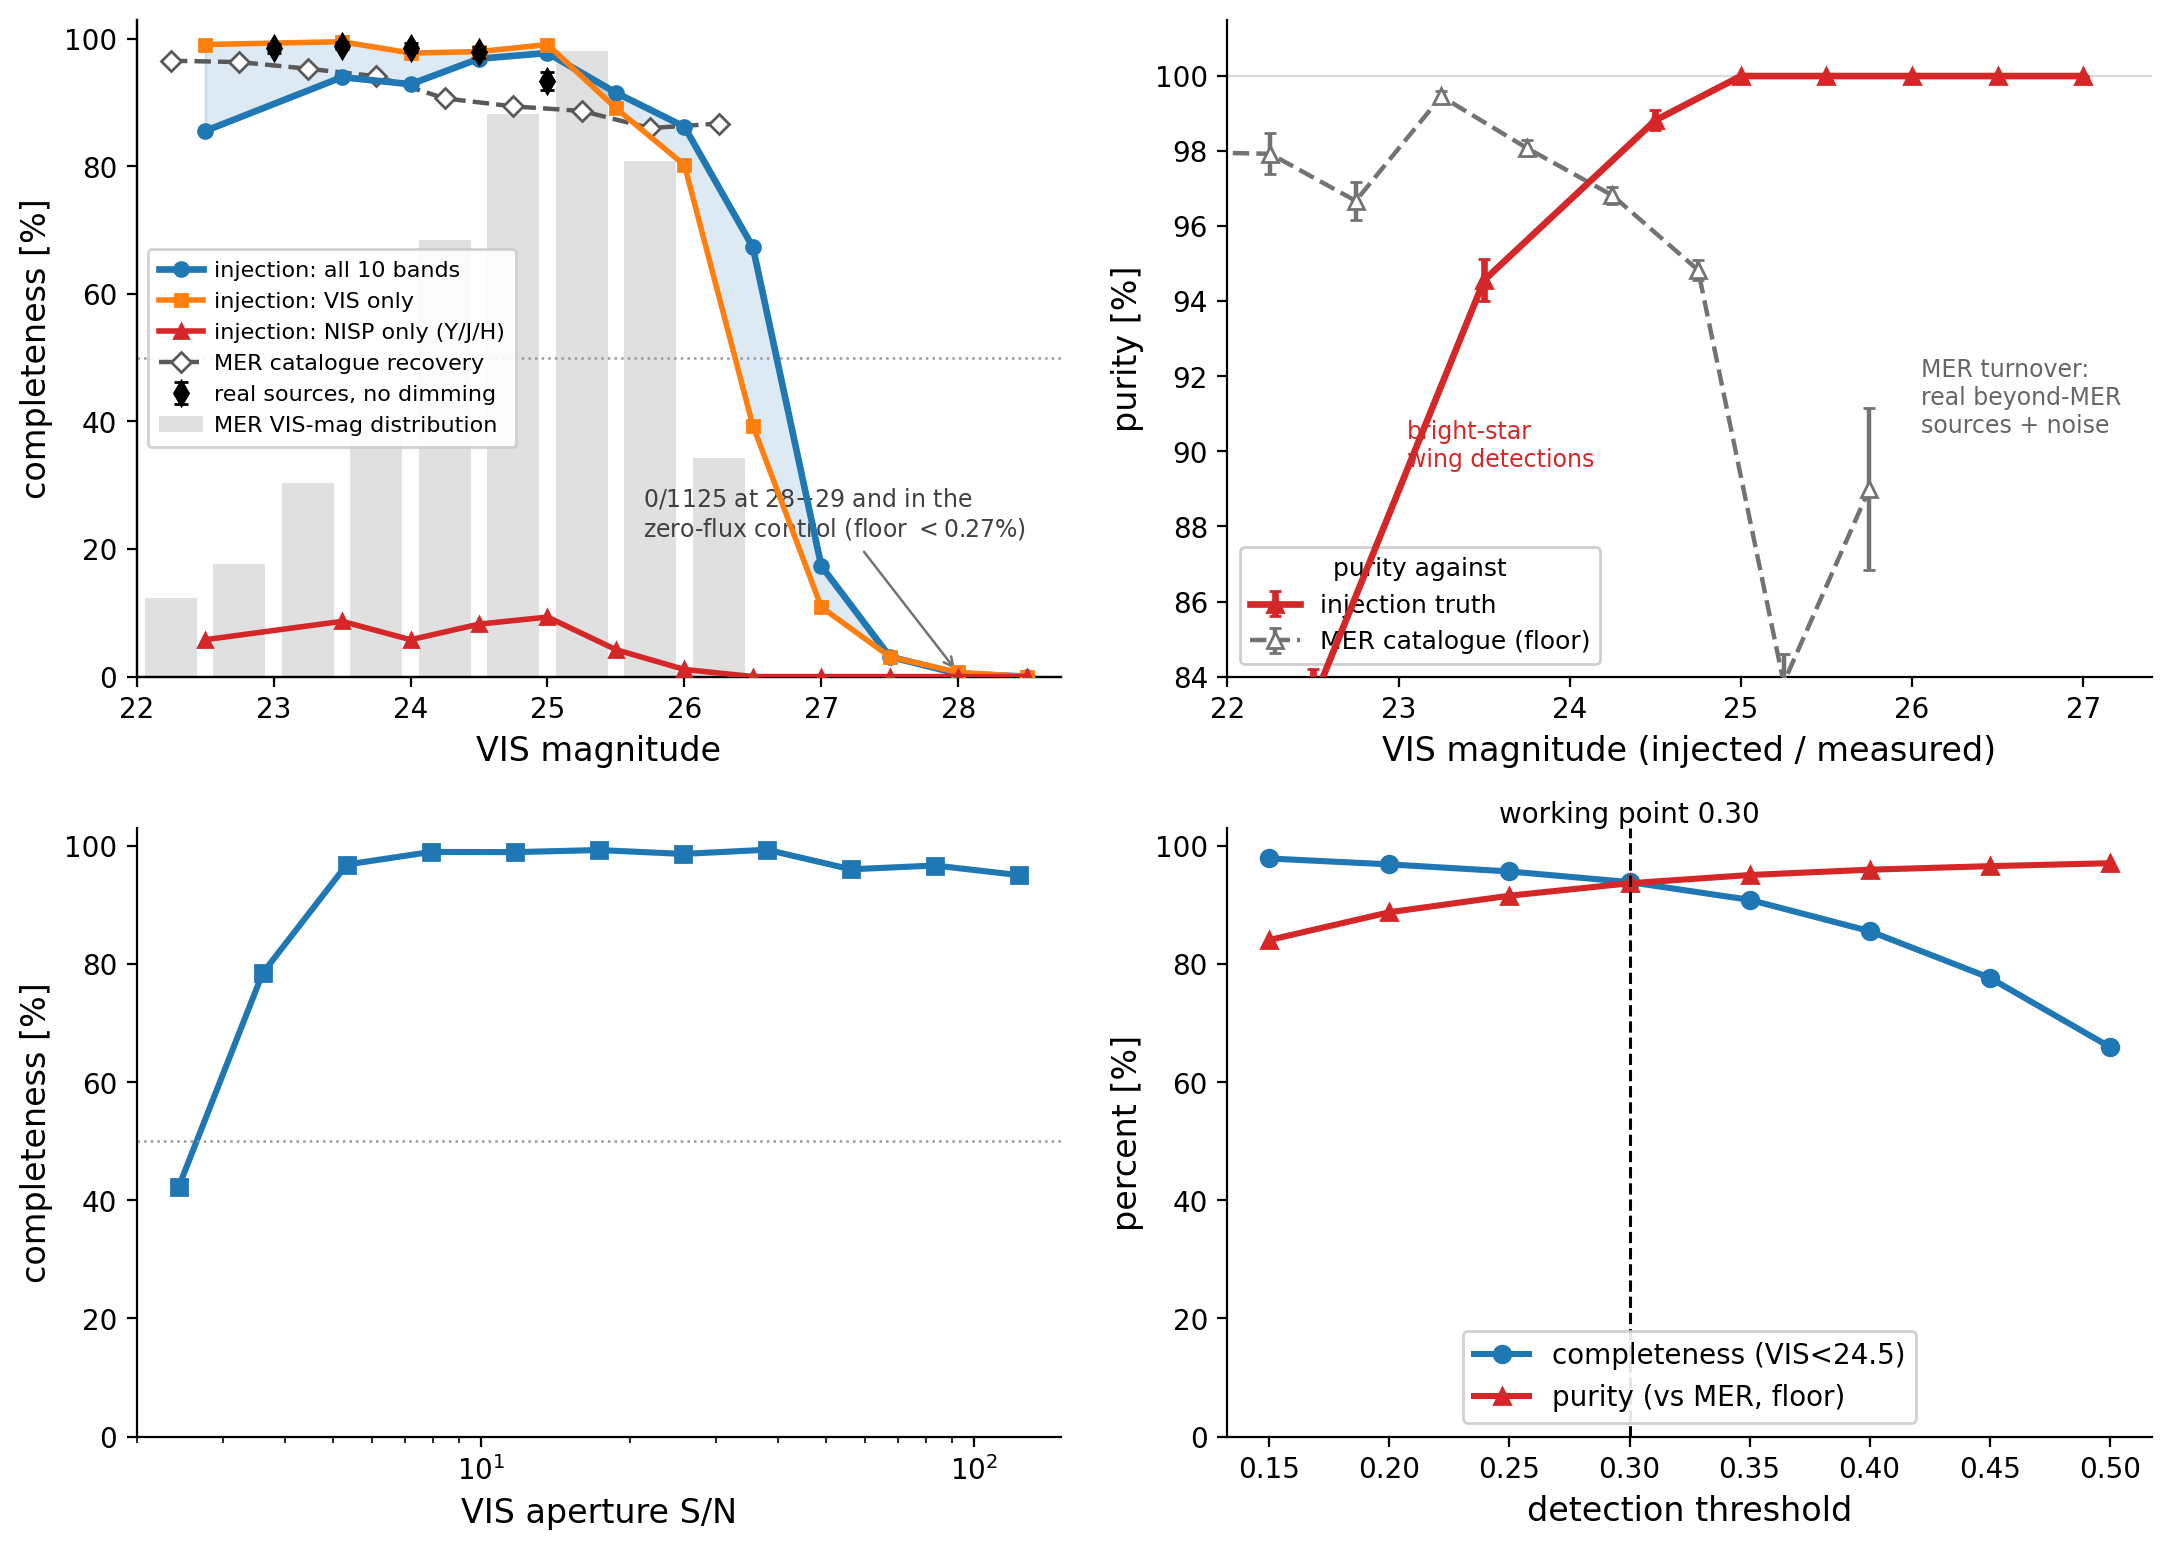
\includegraphics[width=\textwidth]{fig6_detection_performance.png}
    \end{column}
    \begin{column}{0.40\textwidth}
      \vspace{0.5em}
      \begin{itemize}\small\setlength\itemsep{0.6em}
        \item vs.\ MER catalog: \alert{93\% completeness, 95\% purity} (purity a conservative floor).
        \item Catalog-independent injection depth: $50\%$ point-source depth
          \alert{VIS $\approx 25.0$} --- \alert{$+0.45$ mag deeper} than the same detector on VIS alone.
      \end{itemize}
      \vspace{0.3em}
      {\small
      \begin{tabular}{lcc}
        \toprule
        $d_{50}$ (VIS mag) & fused & stems \\
        \midrule
        all 10 bands & $25.0$ & $25.1$ \\
        VIS only     & $24.6$ & $25.1$ \\
        \alert{multi-band gain} & \alert{$+0.45$} & $+0.03$ \\
        \bottomrule
      \end{tabular}}\\[0.4em]
      {\small The gain lives in the \alert{fused representation}, not the head design.}
    \end{column}
  \end{columns}
\end{frame}

% ------------------------------------------------------------ 10
\begin{frame}{Downstream task 2 --- Astrometry: carrying VIS precision to every band}
  \centering
  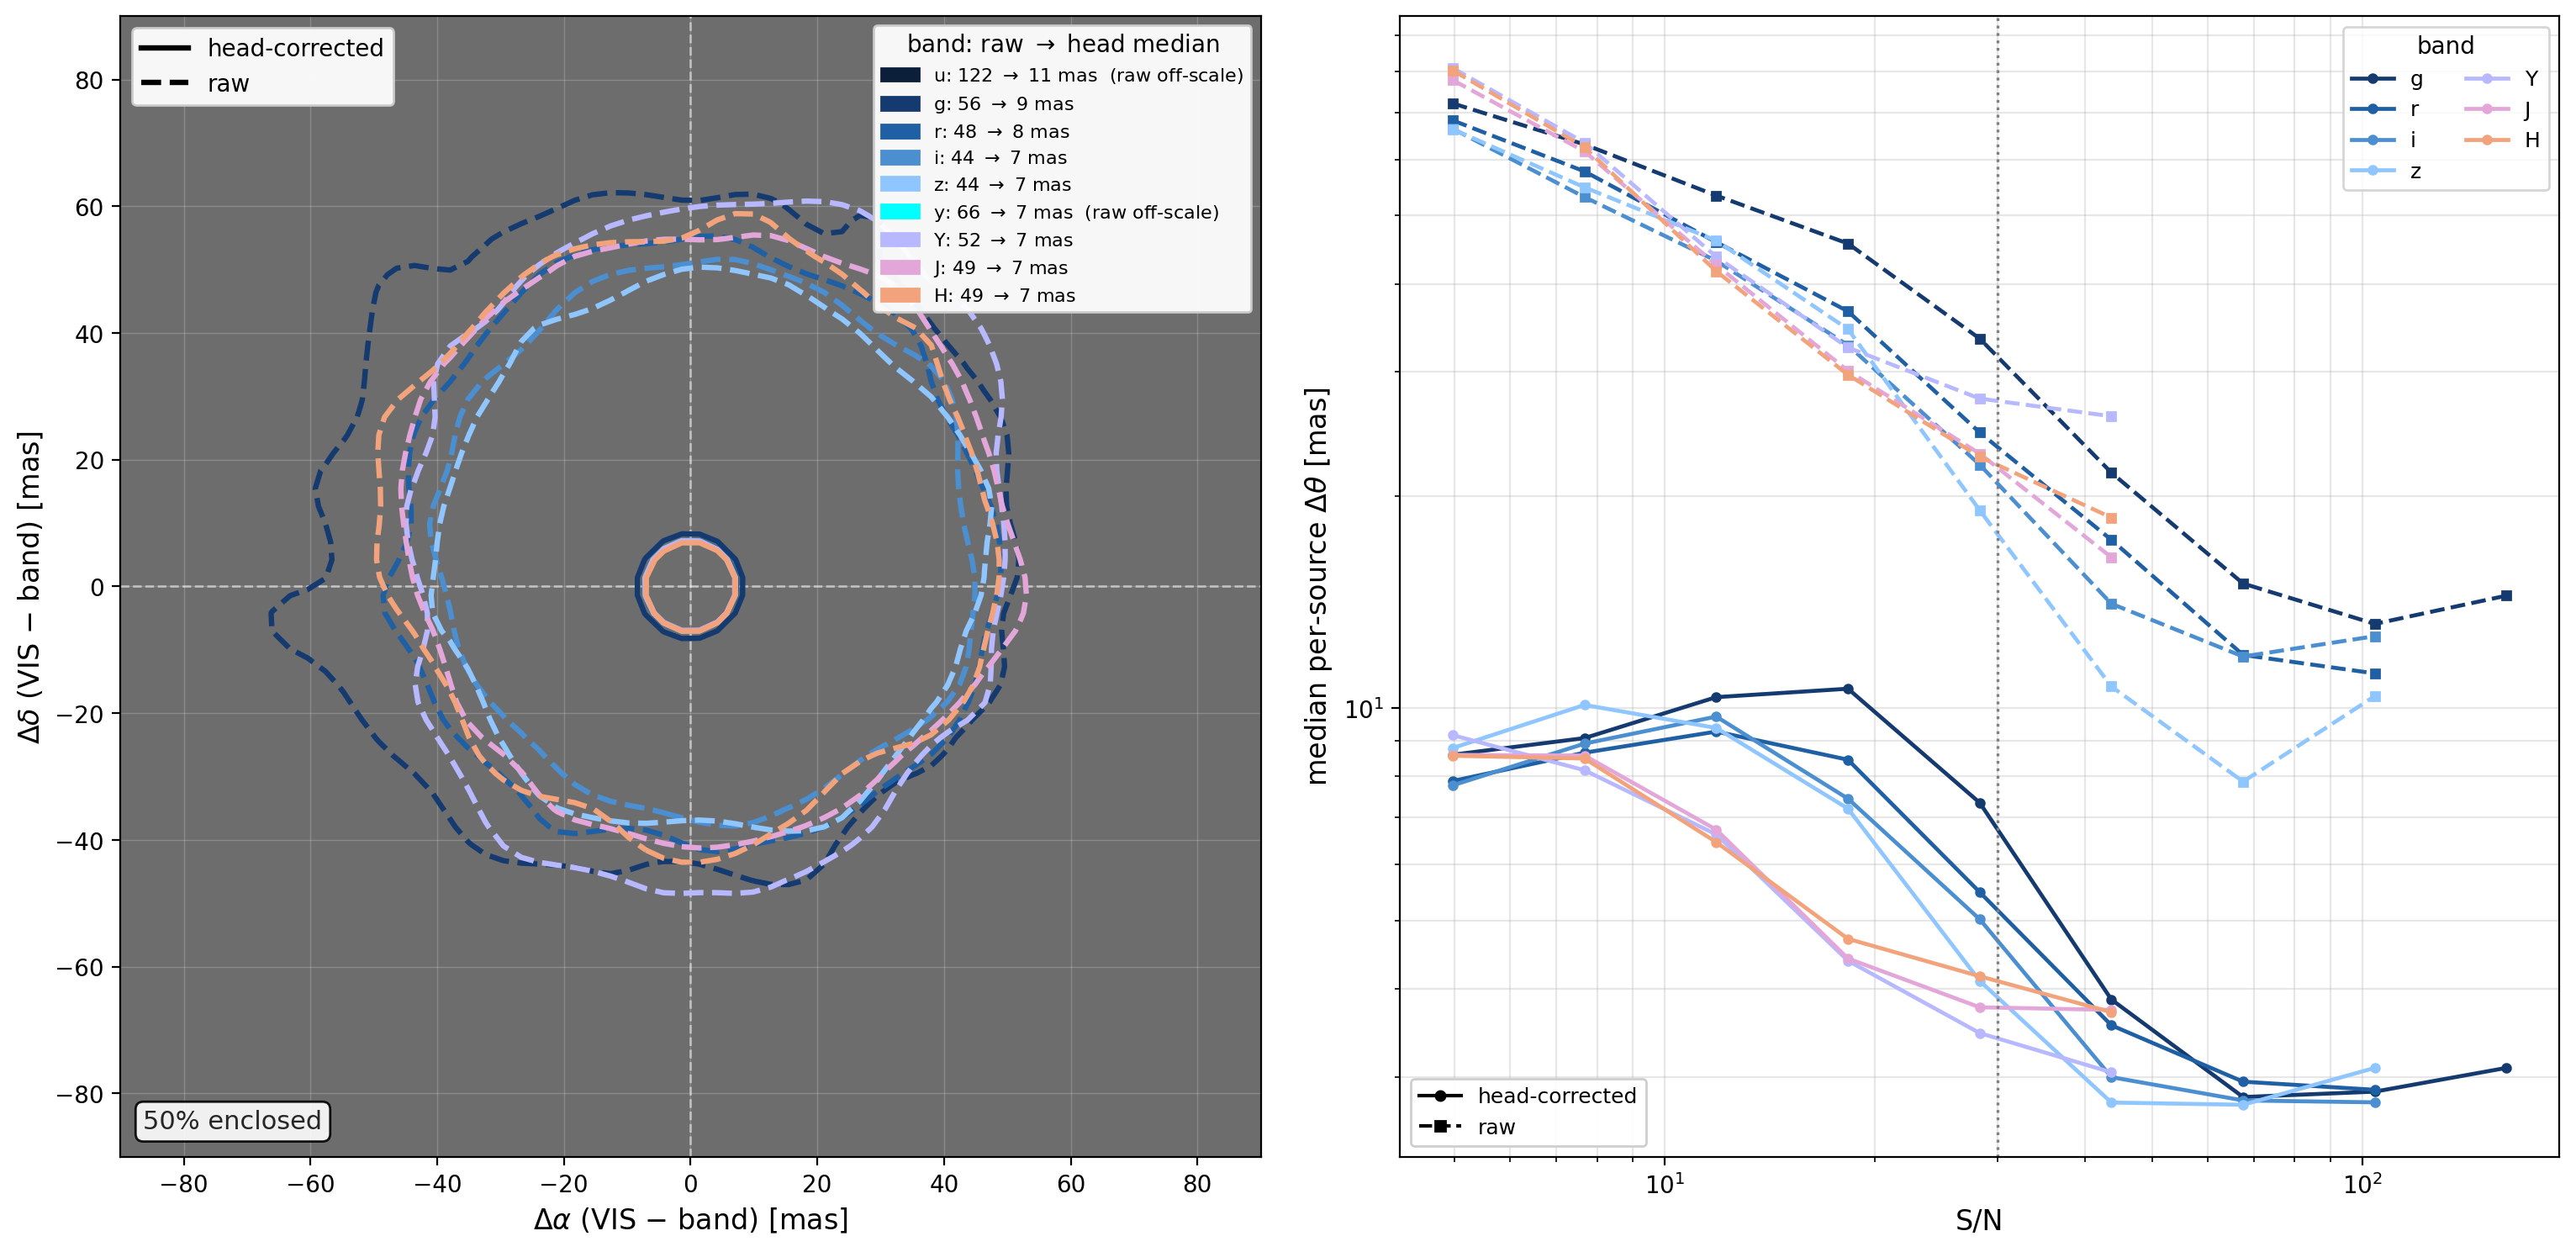
\includegraphics[width=0.76\textwidth]{fig8_head_correction.png}
  \begin{itemize}\small
    \item Raw cross-survey scatter: ${\sim}50\mas$, dominated by photon-noise centroiding of
      faint galaxies. A $0.7$M-parameter position head collapses it to \alert{$14$--$17\mas$}
      and re-centers every band on the origin.
    \item Against \alert{injected truth}: $19\mas$ at $\mathrm{S/N}=5$ vs.\ ${\sim}50\mas$
      classically --- within ${\sim}2\mas$ of the VIS anchor floor. The head carries VIS-quality
      localization to the other nine bands.
  \end{itemize}
\end{frame}

% ------------------------------------------------------------ 11
\begin{frame}{The concordance field: how well do two Gaia-tied surveys actually agree?}
  \centering
  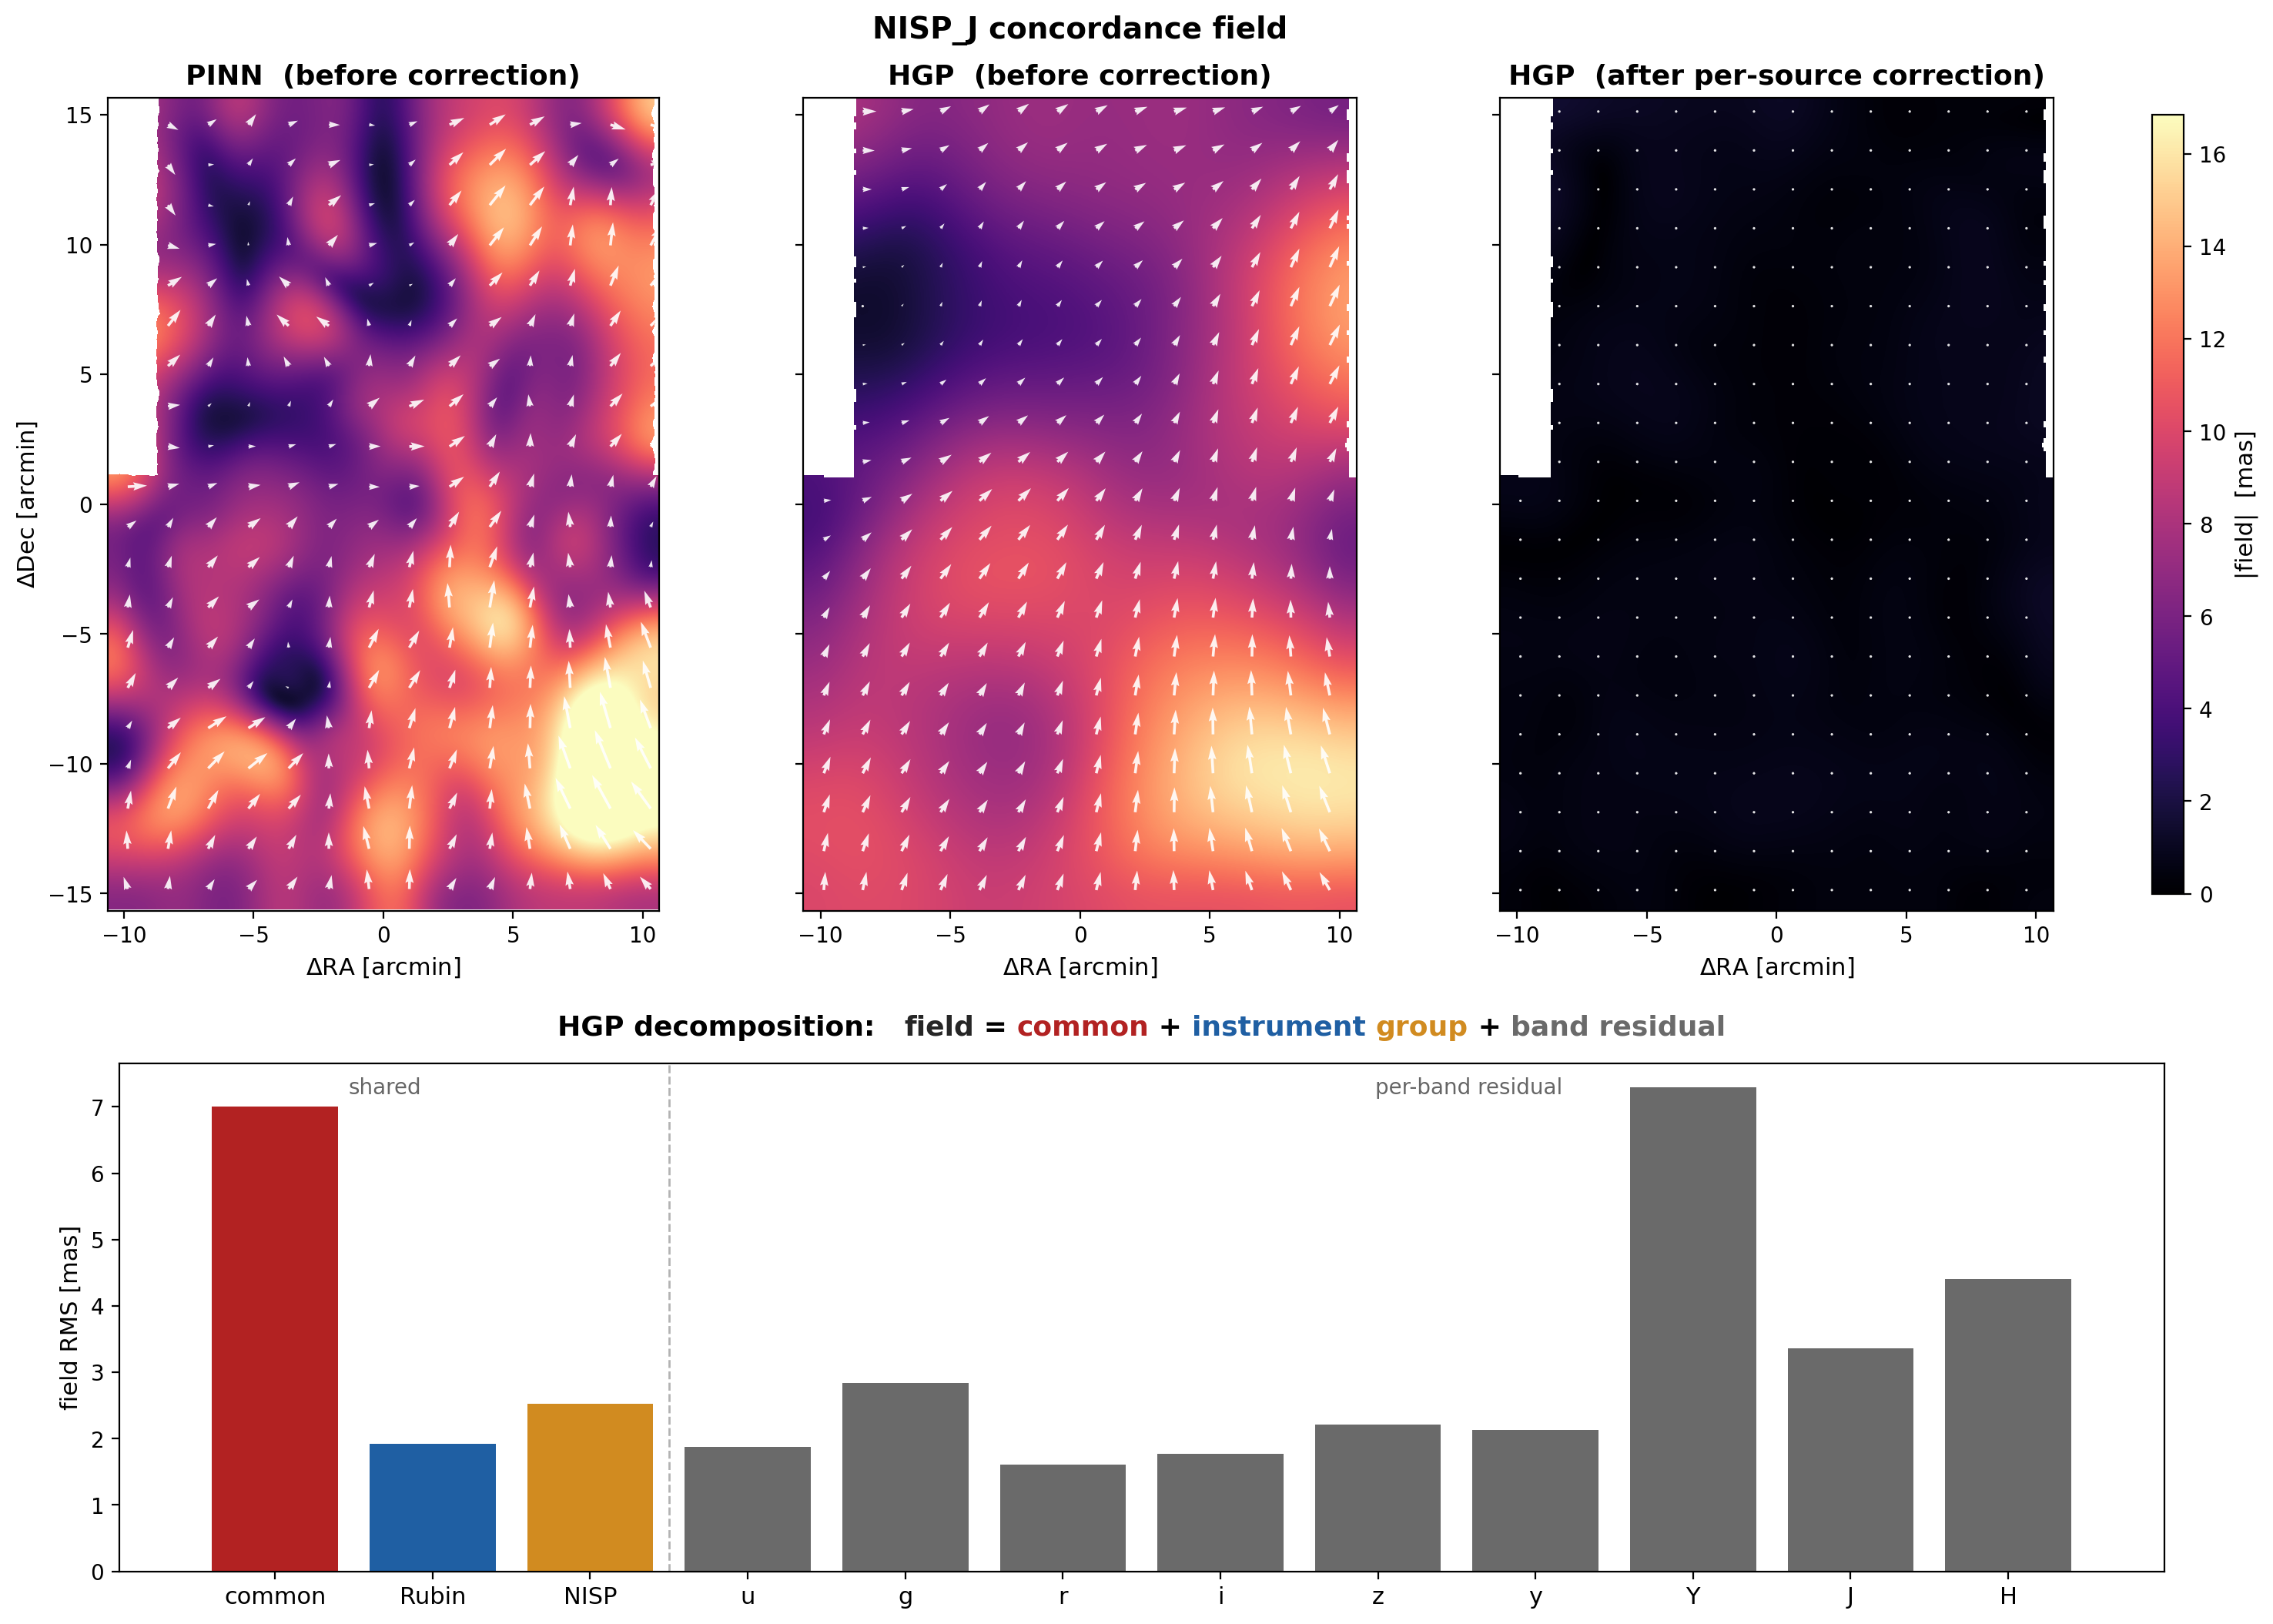
\includegraphics[height=0.60\textheight]{fig10_concordance_field.png}
  \begin{itemize}\small
    \item Beneath the scatter: a coherent \alert{$9$--$10\mas$ pattern} between the two surveys'
      independently Gaia-anchored solutions --- ${\sim}7\mas$ shared by \alert{all ten bands}.
      Recovered by two independent solvers; the head absorbs it source-by-source (${\to}1.5\mas$).
    \item A few-mas, degree-scale \alert{map of cross-survey agreement} --- a QA product for
      joint processing that no single pipeline can produce.
  \end{itemize}
\end{frame}

% ------------------------------------------------------------ 12
\begin{frame}{Does any of this transfer? Zero-shot on a second deep field}
  \centering
  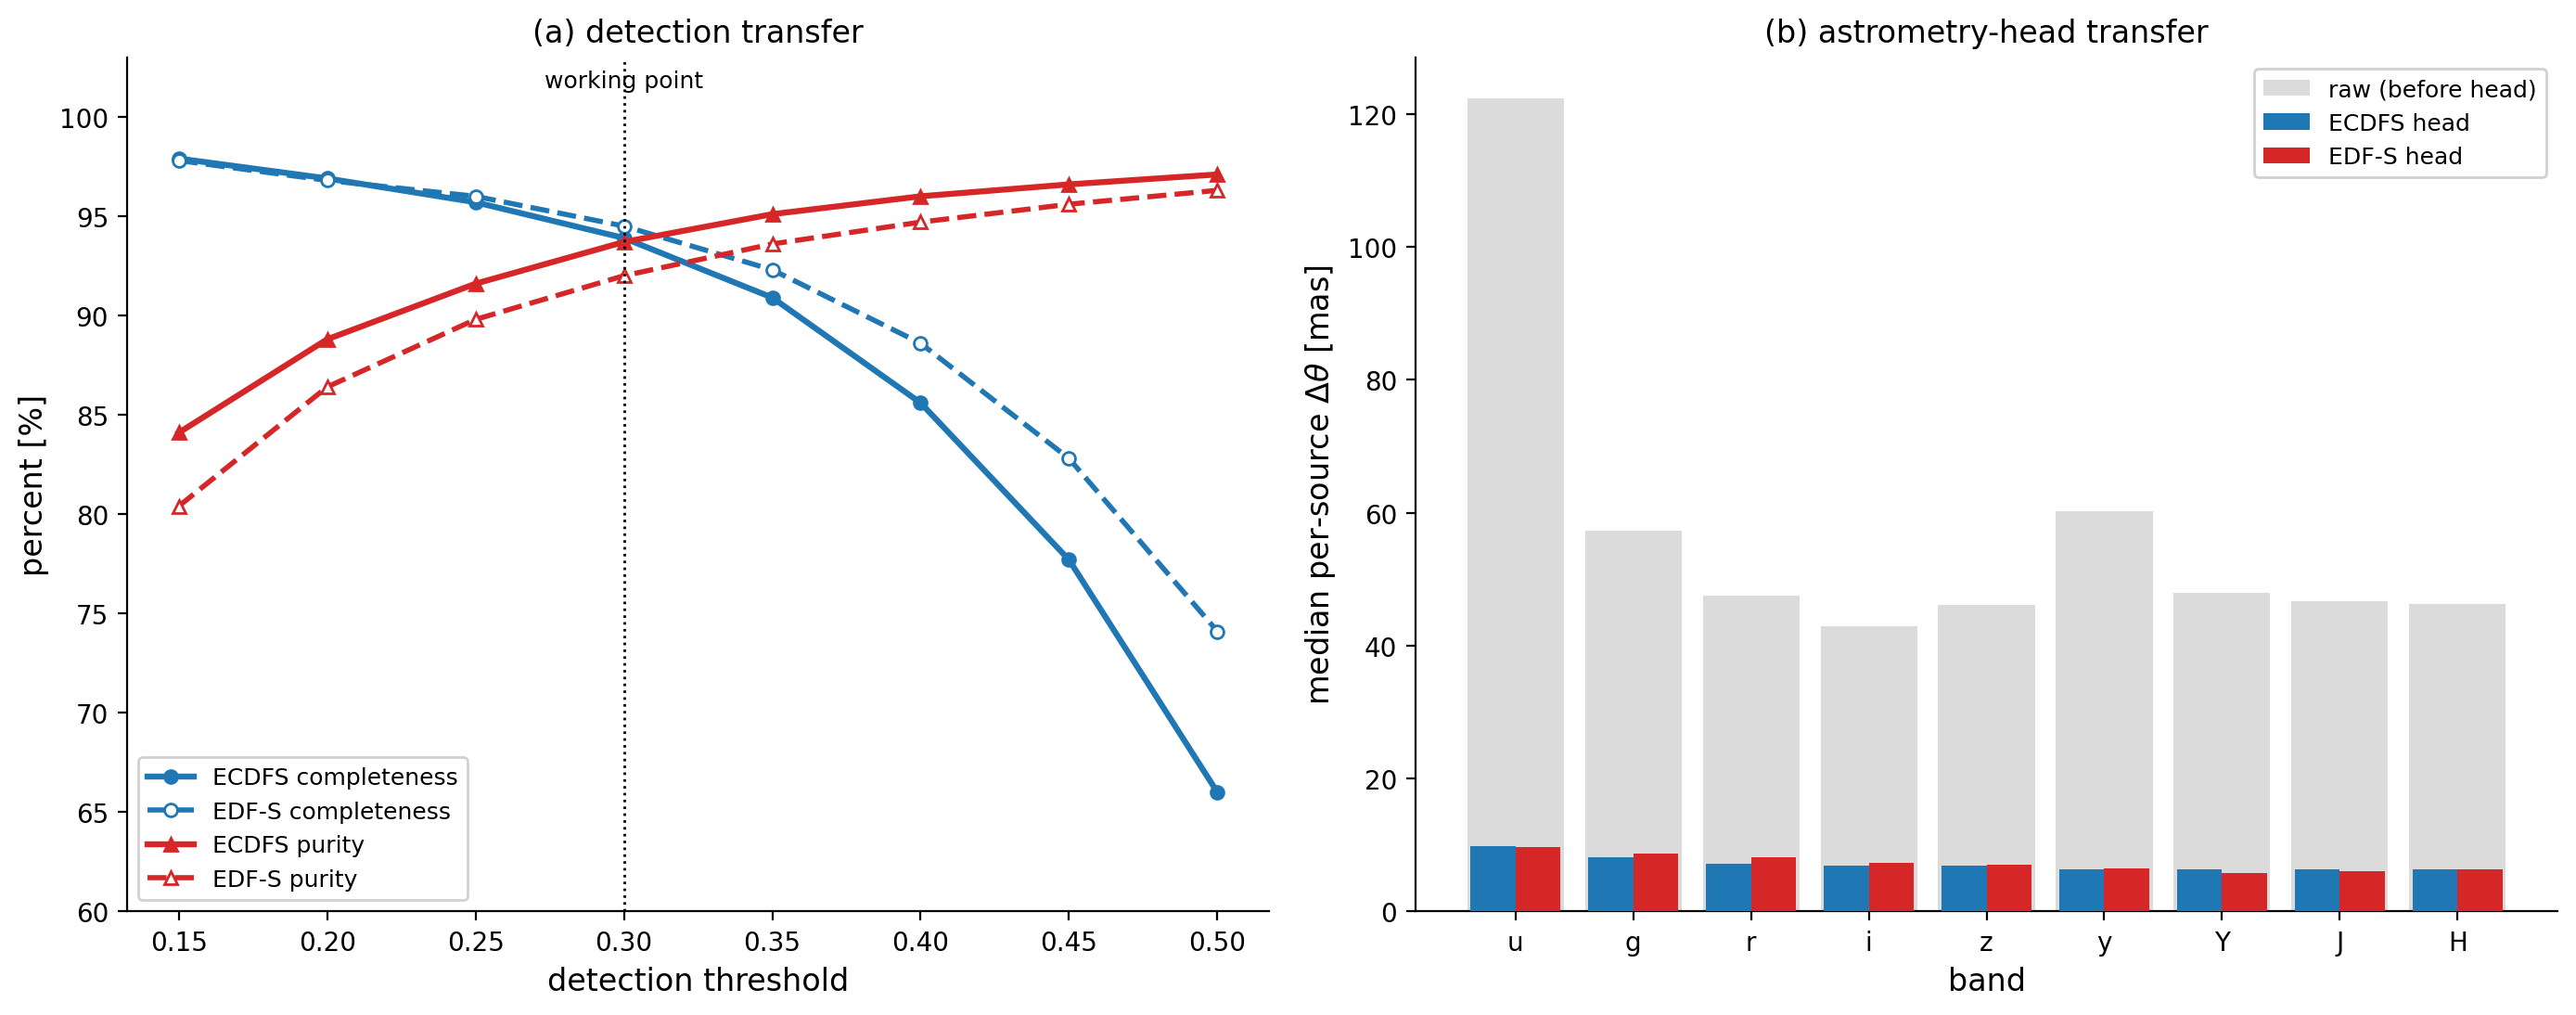
\includegraphics[width=0.88\textwidth]{fig11_ood.png}
  \begin{itemize}\small
    \item Frozen foundation $+$ frozen heads, applied to EDF-S: \alert{nothing retrained}.
    \item Detection: $93.4\%/93.1\%$ completeness/purity vs.\ $93.3\%/94.5\%$ in-distribution.
      Astrometry: same ${\sim}12$--$18\mas$ floor, within $1$--$3\mas$ of the training field.
    \item Scaling to more area is a matter of \alert{applying the stack, not rebuilding it}.
  \end{itemize}
\end{frame}

% ------------------------------------------------------------ 13
\begin{frame}{\textit{Roman}: the natural third stream}
  \begin{columns}[T]
    \begin{column}{0.52\textwidth}
      \textbf{The architecture is built for this:}
      \begin{itemize}\small\setlength\itemsep{0.4em}
        \item one encoder branch per instrument, fused on a common physical grid ---
          \alert{adding \textit{Roman} $=$ adding a third branch}, not redesigning the model
        \item pretraining needs only \alert{overlapping public pixels} --- no labels, no
          simulations; hours of GPU time once WFI imaging overlaps Rubin/\textit{Euclid} sky
      \end{itemize}
      \vspace{0.4em}
      \textbf{What \textit{Roman} brings to the stack:}
      \begin{itemize}\small\setlength\itemsep{0.4em}
        \item \alert{sharp, deep NIR at $0.11''$/px} --- the near-infrared analog of the VIS
          spatial anchor, where today we lean on resampled NISP
        \item wide-area survey over thousands of deg$^2$ \alert{inside the LSST footprint},
          plus deep time-domain fields
      \end{itemize}
    \end{column}
    \begin{column}{0.46\textwidth}
      \textbf{What the joint model does for \textit{Roman}:}
      \begin{itemize}\small\setlength\itemsep{0.4em}
        \item multi-band detection gains beyond any single-band catalog
          (here: $+0.45$ mag from fusion)
        \item WFI-anchored positions carried into Rubin's seeing-limited bands
        \item \alert{three-way concordance fields}: Rubin--\textit{Euclid}--\textit{Roman}
          astrometric agreement mapped at the few-mas level --- systematics QA no
          single pipeline can produce
        \item ingest native-resolution frames and solve cross-instrument registration
          \emph{inside} the model (the ${\sim}3\mas$ NISP resampling residual we detect is
          exactly this kind of inherited error)
      \end{itemize}
      \vspace{0.4em}
      \centering
      \alert{\small Launch window opens August 30 --- the recipe is ready.}
    \end{column}
  \end{columns}
\end{frame}

% ------------------------------------------------------------ 14
\begin{frame}{Takeaways}
  \begin{itemize}\setlength\itemsep{0.9em}
    \item A ${\sim}9$M-parameter foundation model, pretrained \alert{label-free} on public
      Rubin\,$+$\,\textit{Euclid} mosaics in ${\sim}2.5$ GPU-hours, learns a shared ten-band
      representation precise enough for measurement.
    \item \textbf{Detection}: matches the \textit{Euclid} catalog (93\%/95\%), and ten-band fusion
      pushes \alert{$0.45$ mag deeper} than VIS alone.
    \item \textbf{Astrometry}: VIS-quality positions in every band --- ${\sim}50 \to 14$--$17\mas$,
      $19\mas$ at $\mathrm{S/N}=5$ against injected truth --- and a few-mas
      \alert{concordance field} between two Gaia-tied solutions.
    \item The frozen stack \alert{transfers zero-shot} to a second deep field. All of this on the
      \emph{earliest} data both surveys have released --- a floor, not a ceiling.
    \item \textit{Roman} slots in as a \alert{third encoder stream}: sharp NIR anchor, three-way
      cross-survey calibration, and one representation reused across tasks, fields ---
      and instruments.
  \end{itemize}
  \vfill
  \centering
  \srcnote{Hemmati et al.\ 2026 \quad$\cdot$\quad github.com/xoubish/JAISP \quad$\cdot$\quad shemmati@caltech.edu}
\end{frame}

\end{document}
